\documentclass[2dCFT-lecture.tex]{subfiles}

\begin{document}
\section{Minimal models}
This chapter is devoted to the most important class of conformal field theories, called \textbf{minimal models} first studied in the seminal paper \cite[ISZ88-No.1]{belavin1984infinite}. These theories
are characterized by a Hilbert space made of finite numbers of representations of the Verma modules.

\subsection{Conformal family}
From the previous study, we know that primary fields play a fundamental role in conformal field theory. The asymptotic state is given by $\ket{h}=\phi(0)\ket{0}$, which satisfies $L_0 \ket{h}=h\ket{h}$ and $L_n \ket{h}=0$ for  $n>0$. In Verma module section, we also defined descendant states leading by primary $\ket{h}$, by acting a series of $L_{-n}$ on $\ket{h}$. We first study the field operator corresponding to the descendant states. The natural definition of the descendant field associated with the state $L_{-n}\ket{h}$ is
\begin{equation}
\label{def-descendant-field}
\phi^{(- n)} (w) \equiv \left(L _{- n} \phi \right) (w)=\frac{1}{2 \pi i} \oint _{w} d z \frac{1}{(z-w)^{n-1}} T (z) \phi (w)\, .
\end{equation}
By using the OPE \eqref{OPE-T-primaryfield-z}, the above expression can be calculated explicitly.
In particular, we have
\begin{equation}
 \phi^{(0)} (w)=h \phi (w)\, , \quad \text{and} \quad \phi^{(- 1)} (w)=\partial \phi (w)\, .
\end{equation}
Now consider the correlation function with one descendant field in it, i.e.
\begin{equation}
  \left\langle \left(L _{- n} \phi \right) (w) X \right\rangle\, ,
\end{equation}
where $X=\phi _{1} \left(w _{1} \right) \cdots \phi _{N} \left(w _{N} \right)$ is a product of primary fields with conformal dimensions $h_i$.
This correlation function can be calculated by substituting the definition \eqref{def-descendant-field}.
\bea
\label{differential-equation}
 \left\langle \phi^{(- n)} (w) X \right\rangle
 &= \frac{1}{2 \pi i} \oint _{w} d z (z-w)^{1-n} \langle T (z) \phi (w) X \rangle\notag \\
 &=- \frac{1}{2 \pi i} \oint _{\left(w _{i} \right)} d z (z-w)^{1-n} \sum _{i} \{\frac{1}{z-w _{i}} \partial _{w _{i}} \langle \phi (w) X \rangle+ \frac{h _{i}}{\left(z-w _{i} \right)^{2}} \langle \phi (w) X \rangle \}\notag \\
 &\equiv \mathcal{L} _{- n} \langle \phi (w) X \rangle \quad (n \geq 1)\, .
\eea
In the second step, the residue theorem is applied by
reversing the contour including $w$ only and summing
the contributions from all the poles at $w_i$. With
the help of the relevant OPEs, the definition operator $\mathcal{L}_{-n}$ is given by
\begin{equation}\label{L-diff}
 \mathcal{L} _{- n}=\sum _{i} \left\{\frac{(n-1) h _{i}}{\left(w _{i}-w \right)^{n}}-\frac{1}{\left(w _{i}-w \right)^{n-1}} \partial _{w _{i}} \right\}\, .
\end{equation}
This result tells us that the evaluation of a correlation function containing one descendant field
$\phi^{(-n)}$ is controlled by its primary field. $\mathcal{L}_{-1}$ is equivalent to $\partial/\partial{w}$, since the operator
\begin{equation}
\frac{\partial}{\partial w} + \sum _{i} \frac{\partial}{\partial w _{i}}\, ,
\end{equation}
annihilates any correlation functions because of the translation invariance.

The descendant states corresponding to $L_{-k}L_{-n}\ket{h}$ can be defined recursively.
\begin{equation}
\phi^{(- k ,-n)} (w) \equiv \left(L _{- k} L _{- n} \phi \right) (w)
=  \frac{1}{2 \pi i} \oint _{w} d z (z-w)^{1-k} T (z) \left(L _{- n} \phi \right) (w)\, .
\end{equation}
In particular, we have
\begin{equation}
\phi^{(0 ,-n)} (w)=(h + n) \phi^{(- n)} (w) \quad \text{and} \quad
\phi^{(- 1 ,-n)} (w)=\partial _{w} \phi^{(- n)} (w)\, .
\end{equation}
And it can be shown directly that
\begin{equation}\label{descendant-eq}
\left\langle \phi^{\left(- k _{1} \ldots \ldots-k _{n} \right)} (w) X \right\rangle=\mathcal{L} _{- k _{1}} \cdots \mathcal{L} _{- k _{n}} \langle \phi (w) X \rangle\, .
\end{equation}
That is nothing but to apply the differential operators in succession. Consequently, correlation
functions of descendant fields are determined from those of the primary field.  If we obtain all the correlation functions of primary fields in a theory, then the correlation functions, including descendant fields, are thus all determined.

Moreover, all the OPEs with $T(z)$ with descendant states can be calculated in a similar fashion. For example, for
$\phi^{(-1)}=\partial\phi$
\bea
T(z)\partial\phi(w)&\sim \frac{2h\phi(w)}{(z-w)^3}
+\frac{(h+1)\partial\phi(w)}{(z-w)^2}
+\frac{\partial^2\phi(w)}{z-w}\notag\\
&\sim\frac{2\phi^{(0)}(w)}{(z-w)^3}
+\frac{(h+1)\phi^{(-1)}(w)}{(z-w)^2}
+\frac{\phi^{(-1,-1)}(w)}{z-w}\, ,
\eea
where we neglect the regular terms as usual.
The set of a primary field $\phi$
and all of its descendants is called the \textbf{conformal family} of $\phi$, denoted by $[\phi]$. The OPEs with $T(z)$ are closed in the conformal family.





\subsection{Minimal models}\label{sec:MM}
In a conformal field theory (or more generally quantum field theories),
we want to understand correlation functions in the
theory. For free bosons and fermions,
all correlation functions can be calculated by directly using the partition function.
However, it is not so straightforward to determine all the correlation functions for the interacting CFTs.
If there are only finitely many highest weight representations of Virasoro algebra (or finitely many primary fields), one can perform exact computations of correlation functions \cite[ISZ88-No.1]{belavin1984infinite}. Such CFTs are called \textbf{minimal models}.  Let us consider a theory with the set of finitely many highest
weights $\{h_1,\cdots h_p\}$ so that OPEs take the following form:
\begin{equation}\label{op-algebra}
\phi _{1} (z , \overline{z}) \phi _{2} (0,0)
=\sum_p \sum_{\{k,\overline k\}} C^{\{k,\overline k\}}_{12p}
z^{h _{p}-h _{1}-h _{2} + K} \overline{z} ^{\overline{h} _{p}-\overline{h} _{1}-\overline{h} _{2} + \overline{K}}
\phi^{\{k,\overline{k}\}}_p(0,0)\, ,
\end{equation}
where $K=\sum_i k_i$ and $\overline{K}=\sum_i \overline{k}_i$, and $\phi_{i}$ is the primary field with
highest weight $h_i$. As we have seen in the last subsection,  all the correlation functions can be
reduced to the correlation function constructed by
primary fields. Hence, OPEs of primary fields and conformal symmetry completely determine correlation functions if there are only finitely many $p$. In this section, we will learn the method to solve correlation functions in such a model.


\subsubsection*{Kac Determinant}

A representation of the Virasoro algebra is said to be unitary if it contains no negative-norm states. In the section of Verma module, we have mentioned that the negative of central charge and highest weight will make the states non-unitary. As we will see below, the unitarity imposes strong constraints on $(c,h)$.

In addition to unitarity, one has to pay attention to zero-norm states, indeed. If a state $|\chi\rangle$ in a Verma module $V(c,h)$ which is not a highest weight state satisfies the condition
\[
L_n|\chi\rangle=0~, \quad \textrm{for} ~ n>0~,
\]
it is called a \textbf{singular vector}. In fact, a singular vector $|\chi\rangle$ is orthogonal to any state $\prod_i L_{-n_i}|h\rangle$ in the Verma module $V(c,h)$
\[
\langle \chi| \prod_{i}L_{-n_i}|h\rangle=0~.
\]
Therefore, the norm of a singular vector is zero; $\langle\chi|\chi\rangle=0$ so that it is also called a \textrm{null vector} or a \textrm{null state}.

Suppose that there exists a singular vector $|\chi\rangle$ at level $N$ in the Verma module, namely $L_0|\chi\rangle=(h+N)|\chi\rangle$. Then 	its descendants
\[
	L_{-k_1}L_{-k_2}\cdots L_{-k_n}\ket{\chi}\, ,
	\qquad (1\leq k_1 \leq k_2 \cdots \leq k_n)
\]
are all null, and moreover they form a submodule in the Verma module $V(c,h)$. Therefore, in this situation, the Verma module is \textbf{reducible}. In fact, the Verma module $V(c,h)$ is irreducible if and only if it contains no singular vector. Otherwise, an irreducible representation of the Virasoro algebra is
\[
L(c,h)=V(c,h)/J(c,h)
\]
where $J(c,h)$ consists of all null states and their descendants
\[
J(c,h)=\bigcup_{\chi:\textrm{null}}~ \{L_{-k_1}L_{-k_2}\cdots L_{-k_n}\ket{\chi}\}	\qquad (1\leq k_1 \leq k_2 \cdots \leq k_n)
~.
\]



To see if a Verma module has a null state, let us define a Gram matrix as
$M_{ij}=\bra{i}\ket{j}$ where $\ket{i}$ are basis vectors.
For instance, at level two, we have 2 basis
$L_{-2}\ket{h}$, $L_{-1}^2\ket{h}$.
Therefore, the Gram matrix is
\bea
\left(\begin{array}{c c}{\left\langle h \left| L _{2} L _{- 2} \right| h \right\rangle} &{\left\langle h \left| L _{1}^{2} L _{- 2} \right| h \right\rangle} \\{\left\langle h \left| L _{2} L _{- 1}^{2} \right| h \right\rangle} &{\left\langle h \left| L _{1}^{2} L _{- 1}^{2} \right| h \right\rangle} \end{array} \right)=\left(\begin{array}{c c}{4 h + \frac{c}2} &{6 h} \\{6 h} &{4 h (1 + 2 h)} \end{array} \right)\, .
\eea
We focus on a zero eigenvector of this matrix, which gives a linear combination with zero norm. We write the determinant of this matrix as
\begin{equation}
2 \left(16 h^{3}-10 h^{2} + 2 h^{2} c + h c \right)=32 \left(h-h _{1,1} (c) \right) \left(h-h _{1,2} (c) \right) \left(h-h _{2,1} (c) \right)\, ,
\end{equation}
and
\bea\label{level-2}
h _{1,1} (c) &= 0 \cr
h _{1,2}(c)&= \frac{1}{16} (5-c) + \frac{1}{16} \sqrt{(1-c) (25-c)}\cr
h _{2,1} (c)&= \frac{1}{16} (5-c)-\frac{1}{16} \sqrt{(1-c) (25-c)}~.
\eea
The $h=0$ root is actually coming from the null state at level 1, $L_{-1}\ket{0}=0$, which directly implies the vanishing  $L_{-1}(L_{-1}\ket{0})=0$. This is a general feature: if a null state (a state with zero norm) $\ket{h+n}=0$ occurs at level $n$, then at level $N > n$, there are $P(N-n)$ null states $L_{-n_1}\cdots L_{-n_k}\ket{h+n}=0$ (with $\sum_i n_i=N-n$). Thus a null state for some value of $h$ that first appears at level $n$ implies that the determinant at level $N$ will have a $[P(N-n)]$-th order zero for that value of $h$.

At level $N$, the Hilbert space consists of all states of the form
\begin{equation}
\sum _{\left\{n _{t} \right\}} a _{n _{1} \cdots n _{k}} L _{- n _{1}} \cdots L _{- n _{k}} | h \rangle\, ,
\end{equation}
where $\sum _{i} n _{i}=N$.
We can pick $P(N)$ basis states to construct a
$P(N)\times P(N)$ matrix, with the matrix element
as follows.
\begin{equation}
\left\langle h \left| L _{m _{\ell}} \cdots L _{m _{1}} L _{- n _{1}} \cdots L _{- n _{k}} \right| h \right\rangle
\end{equation}
where $\sum _{i=1}^{\ell} m _{i}=\sum _{j=1}^{k} n _{j}=N$. We denote it by
$M_N(c,h)$. If $\det M_N(c,h)$ vanishes, then there exists a linear combination of states with
zero norm for that $c,h$. If negative, then $M_N(c,h)$ has an odd number of negative eigenvalues.
The representation of the Virasoro algebra
at those values of $c$ and $h$ includes states of
negative norm, and is therefore non-unitary.

\begin{figure}[ht]
	\centering
	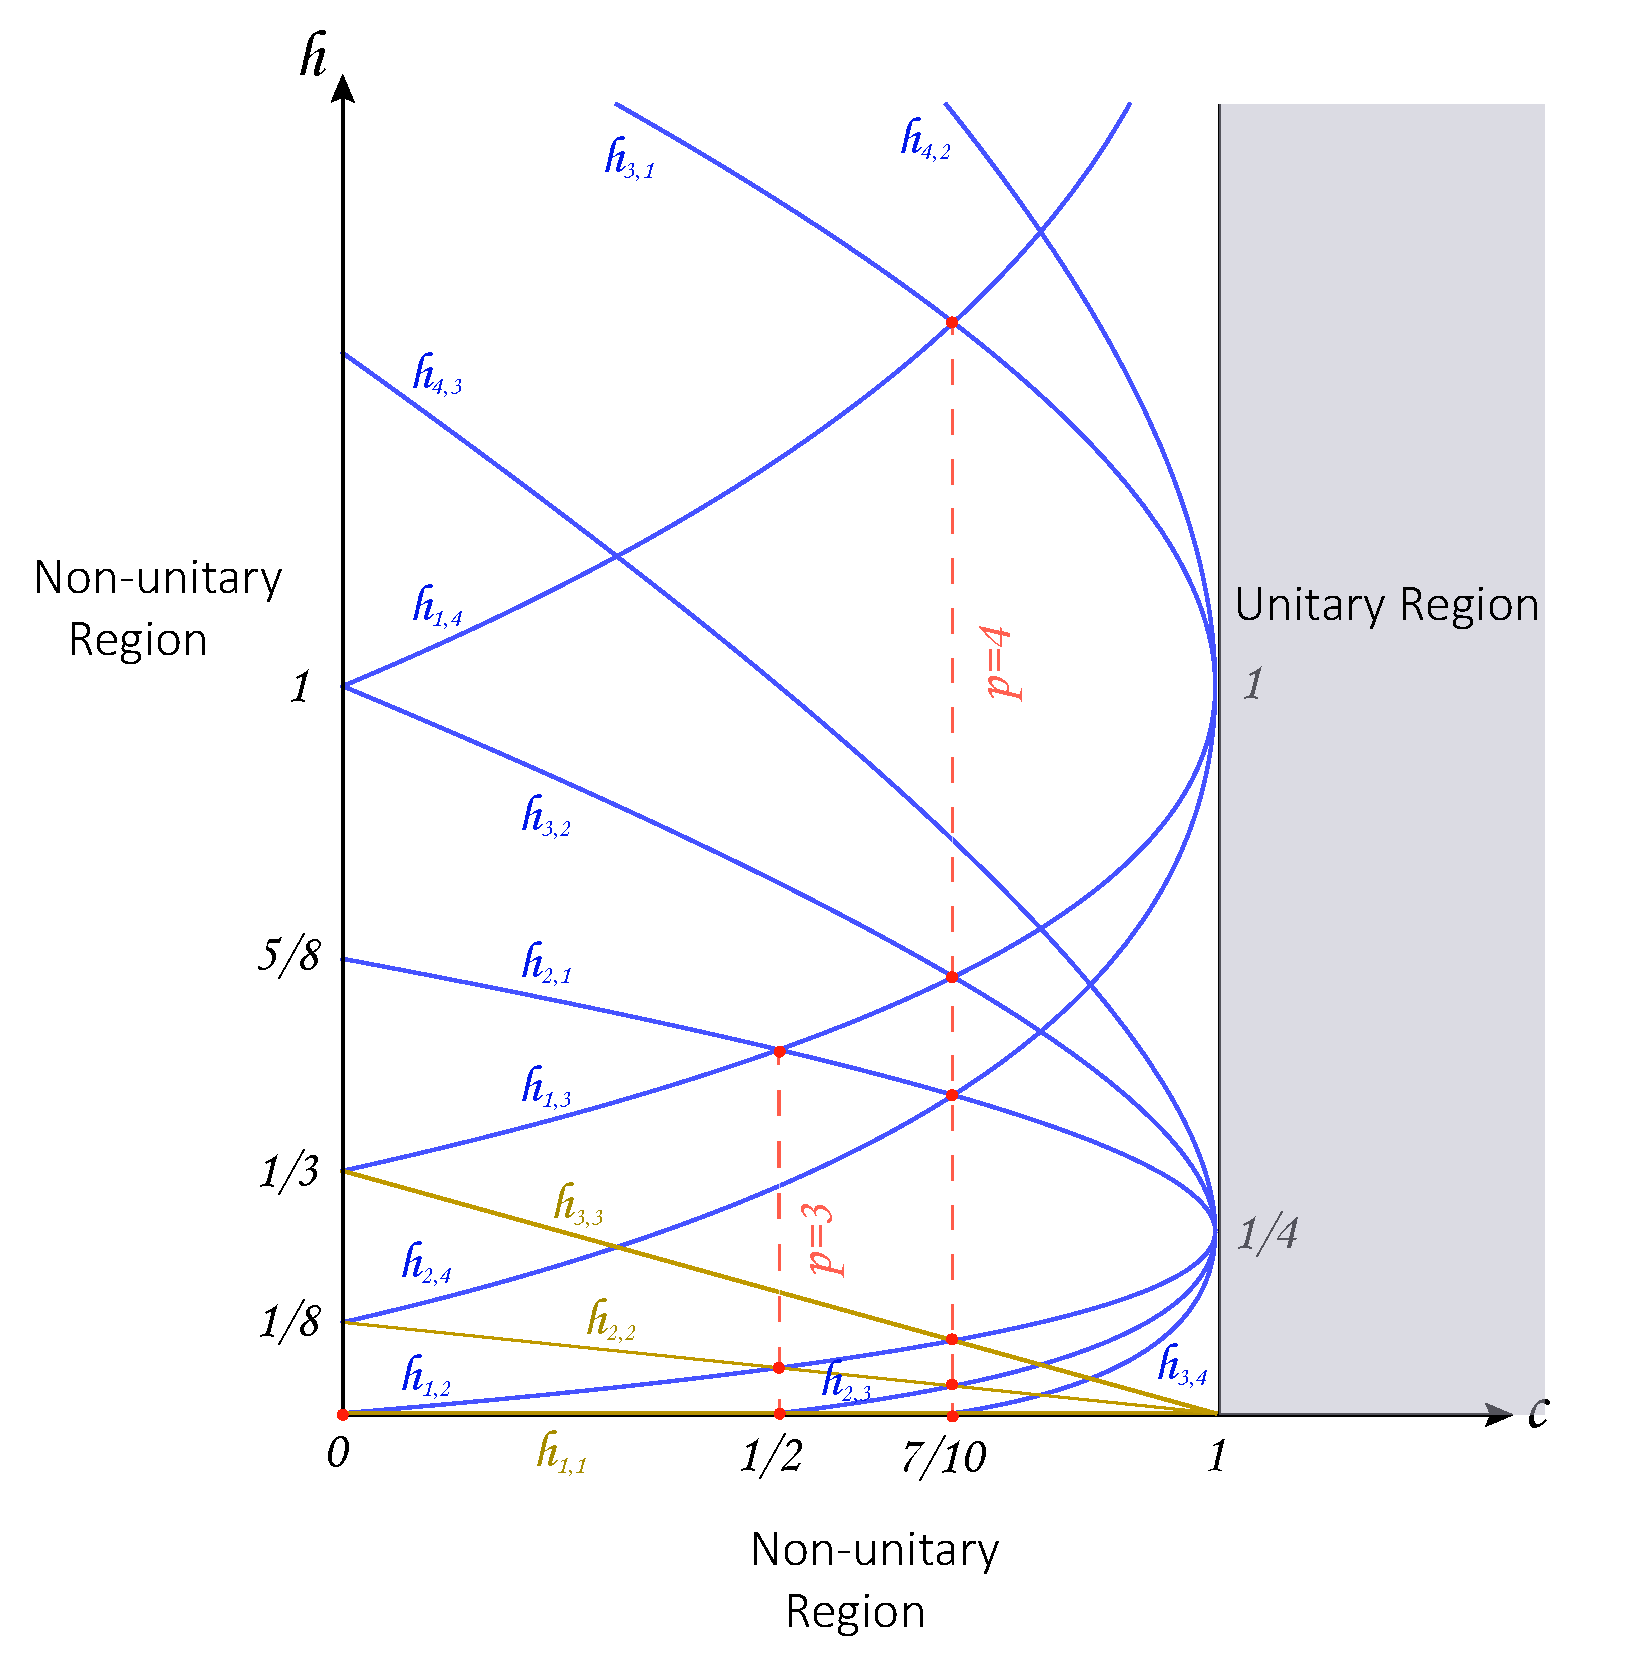
\includegraphics[width=.8\linewidth]{picture/Kac-Determinant}
	\caption{Kac determinant}
	\label{fig:kac-determinant}
\end{figure}

Kac has found a closed form expression of the determinant of $N$ level Gram matrix, which is called \textbf{Kac determinant}  \cite[ISZ88-No.7]{kac1979contravariant}
\begin{equation}
\label{Kac-determinant}
\operatorname{det} M _{N} (c , h)=\alpha _{N} \prod _{r,s  \leq N} \left(h-h _{r,s} (c) \right)^{P (N-rs)}\, ,
\end{equation}
where $\alpha_N$ is a positive constant independent of $c$
and $h$. The Kac determinant provides the complete information of null states in a Verma module.
From this expression, one can see that a null state first appears at level $n=rs$ if $h=h_{r,s}$. Thus at level $N>rs$, the
zero order for $h_{r,s}$ is $P(N-rs)$. In fact, there are two useful equivalent ways to write $h_{r,s}$; the first expression is
\bea
\label{rel-hrs-alpha}
 h _{r,s} (c) &= h _{0} + \frac{1}{4} \left(r \alpha _{+} + s \alpha _{-} \right)^{2}\, ,\notag\\
 h _{0} &= \frac{1}{24} (c-1)\, ,\\
 \alpha _{\pm} &= \frac{\sqrt{1-c} \pm \sqrt{25-c}}{\sqrt{24}}\, ,\notag
\eea
and the second is
\bea
\label{rel-hrs-m}
h _{r,s} (p) &= \frac{[ (p + 1) r-p s ]^{2}-1}{4 p (p + 1)}\, ,\notag\\
c &= 1-\frac{6}{p (p + 1)}\, ,
\eea
where $p$ has two branches
\begin{equation}
\label{m branches}
p=- \frac{1}{2} \pm \frac{1}{2} \sqrt{\frac{25-c}{1-c}}
\end{equation}
From this expression, one can see that when $c=1$, a Verma module is irreducible if $h\neq n^2/4$ for $n\in\bZ$. In addition, when $c=0$, a Verma module is irreducible if $h\neq (n^2-1)/24$ for $n\in\bZ$.

Both of the above expressions provide the following
result for $h_{r,s}(c)$, which is illustrated  in Figure \ref{fig:kac-determinant}
\begin{equation}
\label{rel-hrs}
  h _{r,s} (c)=\frac{1-c}{96} \left[ \left((r + s) \pm (r-s) \sqrt{\frac{25-c}{1-c}} \right)^{2}-4 \right]\, .
\end{equation}
One can convince oneself that $h_{1,2}$ and $h_{2,1}$ are as in \eqref{level-2}.
The Kac determinant changes sign when the values of $(c,h^2)$ cross
each curve $h=h_{r,s}(c)$.



\subsubsection*{Minimal models $\cM_{p,p'}$}
Belavin-Polyakov-Zamolodchikov have noticed that all the correlation functions can be determined by differential equations when the Kac determinant becomes zero.
For example, let us first consider the situation in which there are null states at level two. In general, a null state $\ket{\chi}$ at level two takes the form \begin{equation}
\ket{\chi}=L _{- 2} | h \rangle + a L _{- 1}^{2} | h \rangle \, .
\end{equation}
By applying the $L_1$ to the above equation, we have
\bea
\left[ L _{1} , L _{- 2} \right] | h \rangle + a \left[ L _{1} , L _{- 1}^{2} \right] | h \rangle &= 3 L _{- 1} | h \rangle + a \left(L _{- 1} 2 L _{0} + 2 L _{0} L _{- 1} \right) | h \rangle\notag \\
&= (3 + 2 a (2 h + 1)) L _{- 1} | h \rangle=0
\, ,
\eea
which requires that
\begin{equation}
a=- \frac{3}{2 (2 h + 1)}\, .
\end{equation}
By applying $L_2$, we find that
\bea
\left[ L _{2} , L _{- 2} \right] | h \rangle + a \left[ L _{2} , L _{- 1}^{2} \right] | h \rangle &= \left(4 L _{0} + \frac{c}{2}\right) | h \rangle + 3 a L _{1} L _{- 1} | h \rangle \notag \\
&= (4 h + \frac{c}2 + 6 a h) | h \rangle=0\, .
\eea
Therefore the central charge must satisfy
\begin{equation}
c=2(-6ah-4h)=2h\frac{5-8h}{2h+1}
\end{equation}
Writing $h$ in terms of $c$, we have
\begin{equation}
h=\frac{1}{16}\left\{
5-c\pm \sqrt{(c-1)(c-25)}
\right\}\, ,
\end{equation}
which are equal to $h_{1,2}$ and $h_{2,1}$ in \eqref{level-2}.




Since the null state $\ket{\chi}$ is orthogonal to any states in the Verma module, we have
\begin{equation}
  \label{BPZ}
   \langle \chi (z) X \rangle =0
\end{equation}
where $X$ is a product of arbitrary primary fields as usual. Since $\chi(z)$ can be obtained by acting a linear combination of Virasoro generators \eqref{L-diff} on a primary operator, this equation becomes a linear differential equation for a correlation function of primary fields, called a \textbf{Belavin–Polyakov–Zamolodchikov (BPZ) equation}.
For example, by using
\eqref{differential-equation}, the correlation function
$\expval{\phi(z)X}$ should be governed by the
following differential equation
\begin{equation}
\left\{\mathcal{L} _{- 2}-\frac{3}{2 (2 h + 1)} \mathcal{L} _{- 1}^{2} \right\} \langle \phi (z) X \rangle=0\, ,
\end{equation}
where  $\phi(z)$ has conformal dimension $h_{1,2}$ or
$h_{2,1}$.
One can write the above expression as a differential equation
\begin{equation}
\left\{\sum _{i=1}^{N} \left[ \frac{1}{z-z _{i}} \frac{\partial}{\partial z _{i}} + \frac{h _{i}}{\left(z-z _{i} \right)^{2}} \right]-\frac{3}{2 (2 h + 1)} \frac{\partial^{2}}{\partial z^{2}} \right\} \langle \phi (z) X \rangle=0\, .
\end{equation}
If $X$ is $\phi(w)$ itself, the differential
equation for a two-point function becomes
\begin{equation}
\left\{\frac{1}{z-w} \partial _{w} + \frac{h}{(z-w)^{2}}-\frac{3}{2 (2 h + 1)} \partial _{z}^{2} \right\} \langle \phi (z) \phi (w) \rangle=0\, ,
\end{equation}
which is satisfied by the general form of a two-point function \eqref{two-point-func-form}.
For a three-point function \eqref{three-point-func-form} with $X=\phi_1(z_1)
\phi_2(z_2)$, we have
\begin{equation}
\left\langle \phi (z) \phi _{1} \left(z _{1} \right) \phi _{2} \left(z _{2} \right) \right\rangle=\frac{C_{h,h_1,h_2}}{\left(z-z _{1} \right)^{h+h _{1}-h _{2}} \left(z _{1}-z _{2} \right)^{h _{1}+h _{2}-h} \left(z-z _{2} \right)^{h+h _{2}-h _{1}}}\, .
\end{equation}
The differential equation gives further constraints to
the highest weights of field operators in the three-point function.
\begin{equation}
h _{2}=\frac{1}{6} + \frac{1}{3} h + h _{1} \pm \frac{2}{3} \sqrt{h^{2} + 3 h h _{1}-\frac{1}{2} h + \frac{3}{2} h _{1} + \frac{1}{16}}\, .
\end{equation}
For $h=h_{1,2}$, and set $h_1=h_{r,s}$ in \eqref{rel-hrs}, we find that $h_2$ is equal to $h_{r,s-1}$ or $h_{r,s+1}$. Similarly for $h=h_{2,1}$, $h_2$ is equal to $h_{r-1,s}$ or $h_{r+1,s}$. Recall that the two-point function vanishes unless the two operators have the same conformal dimension. We thus have the following operator algebra
\bea
\phi _{1,2} \times \phi _{r,s} &=[ \phi _{r,s-1} ]+ [\phi _{r,s + 1}]\notag \\
\phi _{2,1} \times \phi _{r,s} &= [\phi _{r-1 , s}] + [\phi _{r + 1 ,s}]\, ,
\eea
where $\phi_{r,s}$ means the field operator with highest weight $h_{r,s}$. The expression above means that the fields $\phi _{1,2}$ and $\phi_{2,1}$ act as ladder operators in the operator algebra. In addition, the field operators expanded in the right side not only contain the primary fields but their descendant fields as well. The coefficient on the right side may be zero. For instance,
\bea
\phi _{1,2} \times \phi _{2,1} &=[ \phi _{2,0} ]+ [\phi _{2,2}]\, ,\notag \\
\phi _{2,1} \times \phi _{1,2} &= [\phi _{0,2}] + [\phi _{2,2}]\, .
\eea
Since the two OPEs are equivalent, this shows the coefficients before $\phi _{2,0}$ and
$\phi _{0,2}$ must be zero.
Therefore, we have
\begin{equation}
\phi _{1,2} \times \phi _{2,1} =[ \phi _{2,2}]\, .
\end{equation}
The above expression can be generalized to
the following fusion rules
\begin{equation}
\label{fusion-rule-1}
\phi_{r_1, s_1}\times \phi_{r_2,s_2}
= \sum_{
	\begin{subarray}{1}
	\quad k=1+\abs{r_1-r_2}\\
	k+r_1+r_2=1\,\text{mod}\, 2
	\end{subarray}
 }^{k= r_1 + r_2 -1}
\,
\sum_{
	\begin{subarray}{1}
	\quad l=1+\abs{s_1-s_2}\\
	l+s_1+s_2=1\,\text{mod}\, 2
	\end{subarray}
}^{l= s_1 + s_2 -1}
[\phi_{k,l}]\, .
\end{equation}
The summation variables $k$ and $l$ are incremented
by $2$. The expression above implies that
the conformal family $[\phi_{r,s}]$ forms a
closed operator algebra.
\begin{figure}
	\centering
	\includegraphics[width=0.6\linewidth]{picture/minimal-model}
	\caption{"diagram of dimensions"}
	\label{fig:minimal-model}
\end{figure}









The operator algebra
\eqref{fusion-rule-1}, implies there are infinitely many conformal families present in the theory.
However, we want a finite set of highest weights in
a minimal model. In order to understand the situation
graphically, we consider the "diagram of dimensions" as in Figure
\ref{fig:minimal-model}.
The points $(r,s)$ in the first quadrant label the various conformal dimensions appearing in the Kac formula.
The dotted line has a slope $\tan\theta=-\alpha_+/\alpha_-$, where $\alpha_{\pm}$ are defined
in \eqref{rel-hrs-alpha}. If $\delta$ is the distance
between a point $(r,s)$ and the dotted line. It is
a good exercise to show the following relation,
\begin{equation}
h _{r , s}=h _{0} + \frac{1}{4} \delta^{2} \left(\alpha _{+}^{2} + \alpha _{-}^{2} \right)\, .
\end{equation}
If the slope $\tan\theta$ is irrational, it will never
go through any integer point $(r,s)$, which means
$\delta$ is always non-zero. There is no periodical
property for $h_{r,s}$. However, if the slope
$\tan \theta$ is rational. That is, if there exist
two coprime integers $p$ and $p'$ such that
\begin{equation}
p^{\prime} \alpha _{-} + p \alpha _{+}=0\, .
\end{equation}
The dotted line will go through the point $(p',p)$, we
have the following periodicity property.
\begin{equation}
h _{r, s}=h _{r + p, s + p^{\prime}}\, .
\end{equation}
Therefore, there are finitely many primary fields and we call it the \textbf{minimal model} denoted by $\cM_{p,p'}$.
Using \eqref{rel-hrs-alpha}, the central charge and
the Kac formula become
\bea
\label{minimal_model}
c &= 1-6 \frac{\left(p-p^{\prime} \right)^{2}}{p p^{\prime}}\notag \, ,\\
h _{r , s} &= \frac{\left(p^{\prime} r-p s \right)^{2}-\left(p-p^{\prime} \right)^{2}}{4 p p^{\prime}}\, .
\eea
We can obtain a symmetry property from above:
\begin{equation}\label{inversion-formula}
h _{r , s }=h _{p -r, p^{\prime}-s}\, .
\end{equation}
Now, we get a finite set of conformal families, which
closes under fusion rules. The corresponding finite
set of conformal dimensions $h_{r,s}$ is given by
$1\leq r < p$ and $1 \leq s < p^{\prime}$. The symmetry above
gives
\begin{equation}
\phi _{r , s}=\phi _{p-r , p^{\prime}-s }\, .
\end{equation}
Hence, there remain $(p-1)(p'-1)/2$ distinct fields in the
theory.
And the fusion rule is modified to be
\begin{equation}\label{MM-fusion}
\phi _{r,s}\times\phi _{m,n}=
\sum^{k_{\text{max}}}_{
\begin{subarray}{1}
  \quad  k=1+ \abs{r-m} \\
  k+r+m=1 \, \text{mod} \, 2
\end{subarray}}
\,
\sum^{l_{\text{max}}}_{
	\begin{subarray}{1}
	\quad  l=1+ \abs{s-n} \\
	k+s+n=1 \, \text{mod} \, 2
	\end{subarray}}
\left[\phi _{k,l}\right]\, ,
\end{equation}
where the upper bound of the summation now is control
by the periodical and symmetric condition.
\bea
k _{\max} &= \min \left(r + m-1,2 p -1-r-m \right)\, ,\\
l _{\max} &= \min (s + n-1,2 p^{\prime}-1-s-n)\, .
\eea
We will see several examples of minimal models in the following subsections.





























\subsubsection*{Unitarity for $c> 1$}

A representation of the Virasoro algebra is unitary if it contains no negative-norm states.
We can further use Kac determinant to derive the unitarity condition.
In fact, the unitary condition gives us a strong constraint of
the choice of $h$ and $c$, especially in the
region $0\le c\le1$.





We now sketch the proof that the representations are unitary when $(c>1,h>0)$. The proof is separated into three steps as follows:

The first step is to prove that for each curve $C_{r,s}: h= h_{r,s}$, it will either be located below, or on the axis $h=0$ if $c>1$. If $1<c<25$, from \eqref{rel-hrs}, $h_{r,s}$ is not real unless $s=r$, where $h_{r,s}\leq0$. If $c\geq 25$ the choice \eqref{m branches} implies that $-1<p<0$. Then $p(p+1)<0$ and $[(p+1)r-ps]\geq 1$. According to \eqref{rel-hrs-m}, this tells us $h_{r,s}(p)$ is
not positive.  Thus we finish our proof for the first step.

The second step is to prove that the Kac determinant is positive throughout the region.
For a given level, we can find a $h$ larger than any $h_{r,s}$, and at such a point Kac determinant is positive. Since none of the curves lies in the region, the determinant sign can not be changed throughout the region by crossing any curves. This proves the second point.

The last step is to prove that the Gram matrix at level $N$, $M_N$ is positive definite in this region, which is equivalent to the theory
in this region is unitary. Since the Kac determinant is positive, we have even number of negative eigenvalues of $M_N$. Since this number can change only across one of the curves $C_{r,s}$, and is consequently fixed to be the same in the region. Therefore, we need to show that the matrix $M_N$ for each level $N$ is positive definite for at least one point $(c,h)$ in the region.

In order to do this, we define the length $n(\alpha)$ of a basis vector $\ket{\alpha}$ as the number of operators $L_k$ acting on the primary state $\ket{h}$. For instance,
$L^{3}_{-1}$ has length $3$ and $L_{-3}\ket{h}$ has length 1. It is possible to show that the dominant behavior in $h$ of inner products is
\bea
  \langle \alpha | \alpha \rangle &= c _{\alpha} h^{n (\alpha)} [ 1 + \cO (1 / h) ] \quad \left(c _{\alpha} > 0 \right)\cr
  \langle \alpha | \beta \rangle &= \cO(h^{(n (\alpha) + n (\beta)) / 2-1}) + \ldots
  \, .
\eea
where $\ket{\alpha}$ and $\ket{\beta}$. The above expression immediately shows that $M_N$ is dominant by its diagonal element when $h$ is sufficiently large, and thus $M_N$ is positive definite. Therefore, in this region, a Verma module $V(c,h)$ is irreducible.

\subsubsection*{Unitarity for $0 \le c \le 1$}
In this region, we just roughly give some statements. First, it is easy to show that, in Figure \ref{fig:kac-determinant},  any two points in the region $0\le c\le1$, $h>0$ to the $c>1$ region can be connected by a path that passes a single vanishing curve of the Kac determinant at some level. The determinant changes its sign while crossing the vanishing curve. There must be a negative norm state at that level. Therefore, no unitary representations of the Virasoro algebra are allowed in this region, except those on the vanishing curves themselves. A more careful analysis tells us that there is an additional negative norm state everywhere on the vanishing curves except at certain points where they intersect.

Therefore, the unitary representations of the Virasoro algebra only occur at the values of the central charge \cite[ISZ88-No.3]{Cardy:1984bb}:
\begin{equation}
\label{c<1-unitary-c}
c=1-\frac{6}{p (p + 1)} \, ,\quad p=3,4 , \ldots
\end{equation}
with the corresponding highest weight
\begin{equation}
\label{c<1-unitary-hrs}
h _{r,s} (p)=\frac{[ (p + 1) r-p s ]^{2}-1}{4 p (p + 1)}\, .
\end{equation}
where $r,s$ satisfies $1 \leq s \leq r \leq p-1$. The form is exactly the same as \eqref{rel-hrs-m}, but now $p$ can only take discrete integers. This result tells us that the unitary condition is satisfied only at the point $(c,h)$ where the Verma module has null states.

\subsubsection*{Unitary Minimal Models $\cM_p$}
We now consider the choice of $p$ and $p'$ to make the minimal models unitary. Recalling the admissible conformal dimensions in \eqref{minimal_model}, Bezout's lemma states that there exists a couple of integers $(r_0,s_0)$ in the range $1\leq r_0 < p$ and $1 \leq s_0 < p^{\prime}$ such that
\begin{equation}
p^{\prime} r _{0}-p  s _{0}=1\, .
\end{equation}
Thus, the corresponding conformal dimension
\begin{equation}
h _{r _{0} , s _{0}}=\frac{1-\left(p-p^{\prime} \right)^{2}}{4 p p^{\prime}}
\, ,
\end{equation}
which is always negative, expect if $\abs{p-p'} =1$, in which case it vanishes. In fact, the minimal model is unitary only if $\abs{p-p'} =1$, and the primary field $h _{r _{0} , s _{0}} =0$ is indeed the identity operator. Hence, we can set $p'=p+1$ so that the central charge is expressed in \eqref{c<1-unitary-c}. We denote the unitary minimal model by $\cM_p$. We note that the list of unitary representations given in \eqref{c<1-unitary-c} and \eqref{c<1-unitary-hrs}, coincides with the list of highest weight $h_{r,s}$ of unitary minimal models.




\subsection{Characters of minimal models}\label{sec:characters-MM}
The character of an irreducible representation of the Virasoro algebra
\[
\chi _{h} (\tau) \equiv \operatorname{Tr} _{L(c,h)} q^{L _{0} -\frac{c}{24}}=q^{-\frac{c}{24}} \sum _{N=0}^{\infty} d _{h} (N) q^{h + N}~,
\]
where $d_h(N)$ is the number of states at level $N$, and $d_h(N)\le P(N)$. If there is no null state, $d_h(N)=P(N)$. As seen \eqref{character-decomp},
the torus partition function with periodic boundary conditions is
\bea
Z _{\mathrm{PP}} (\tau , \overline{\tau}) &= \operatorname{Tr}_{\cH} \left(q^{L _{0}-\frac{c}{24}} \overline{q}^{\overline{L} _{0}-\frac{c}{24}} \right)\cr
&= \sum _{h , \overline{h}} \mathcal{N} _{h \overline{h}} ~\chi _{h} (\tau) \chi _{\overline{h}} (\overline{\tau})~,
\eea
where $ \mathcal{N} _{h \overline{h}} $ is the number of primary fields of conformal dimension $(h,\overline h)$ \cite[ISZ88-No.25]{cardy1986operator}. Since there is only one vacuum, we set $\cN_{00}=1$. Under the $T$-transformation, a character behaves as
\be\label{T-trans}
\chi _{h} (\tau + 1)=e^{2 \pi i (h-\frac{c}{24})} \chi _{h} (\tau)~.
\ee
The invariance of $\cZ_{\mathrm{PP}}$ under the $T$-transformation requires
\[\mathcal{N} _{h \overline{h}}=0 , \quad h-\overline{h} \notin \mathbb{Z}~.\]
If we write the $S$-transformation of characters
\[\chi _{h} (-1/\tau)=\sum _{h^{\prime}} S _{h h^{\prime}} ~\chi _{h^{\prime}} \left(\tau \right)~,\]
then the modular invariance of $\cZ_{\mathrm{PP}}$ requires
\begin{equation}
\label{relation N S}
\sum _{h , \overline{h}} \mathcal{N} _{h \overline h} S _{h h'} S _{\overline{h} \overline{h}^{\prime}}=\mathcal{N} _{h^{\prime} \overline{h}^{\prime}}~.
\end{equation}
Below we will determine the partition function of diagonal type $\cN_{hh'}=\delta_{hh'}$ in the unitary minimal models. We will see one example of non-diagonal type in the tricritical Ising model in \S\ref{sec:examples}, and the classification of the modular invariant partition functions is discussed at the end of \S\ref{sec:su2k-character}.

From the Kac determinant, we have learned that the Verma module $V_{h_{r,s}}$ has a singular vector at level $rs$. Since $h_{r,s}+rs=h_{-r,s}$, the singular vector generates a submodule $V_{h_{-r,s}}$. Furthermore. since $h_{p-r,p'-s}+ (p-r) (p'-s)=h_{2p-r,s}$, we have another submodule $V_{h_{2p-r,s}}$. Moreover, these submodule $V_{h_{-r,s}}$, $V_{h_{2p-r,s}}$ contain other submodules $V_{h_{-2p-r,s}}$, $V_{h_{2p+r,s}}$, and one can see repeatedly this pattern \cite[ISZ88-No.9]{feigin1983verma}.


\begin{figure}[ht]
\centering
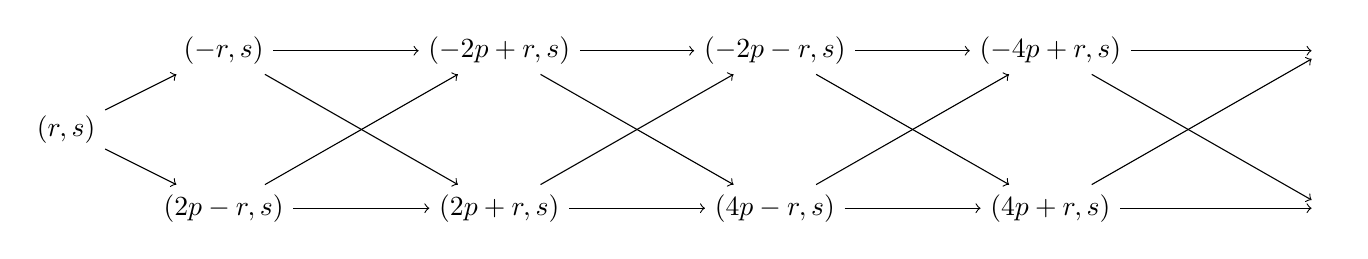
\begin{tikzpicture}[node distance=3.5cm]
\node (A) at (0,0){$(r,s)$};
\node (B) at (2,1){$(-r,s)$};
\node (C) at (2,-1){$(2p-r,s)$};
\node [ right of =B] (D){$(-2p+r,s)$};
\node [ right of =D] (E){$(-2p-r,s)$};
\node [ right of =E] (F){$(-4p+r,s)$};
\node [ right of =F] (F1){$\ $};
\node [ right of =C] (G){$(2p+r,s)$};
\node [ right of =G] (H){$(4p-r,s)$};
\node [ right of =H] (I){$(4p+r,s)$};
\node [ right of =I] (I1){$\ $};
\draw[->] (A) -- (B);
\draw[->] (A) -- (C);
\draw[->] (B) -- (D);
\draw[->] (D) -- (E);
\draw[->] (E) -- (F);
\draw[->] (C) -- (G);
\draw[->] (G) -- (H);
\draw[->] (H) -- (I);
\draw[->] (F) -- (F1);
\draw[->] (I) -- (I1);
\draw[->] (B) -- (G);
\draw[->] (D) -- (H);
\draw[->] (E) -- (I);
\draw[->] (C) -- (D);
\draw[->] (G) -- (E);
\draw[->] (H) -- (F);
\draw[->] (F) -- (I1);
\draw[->] (I) -- (F1);
\end{tikzpicture}
\end{figure}



Therefore, the character of the irreducible representation $L(c,h_{r,s})$ of the Virasoro algebra is
\begin{align} \chi _{r, s} (\tau) &=\operatorname{Tr} _{L(c,h_{r,s})} q^{L _{0} -\frac{c}{24}} \cr
  &=\frac{1}{q^{-\frac124}\eta (\tau)} q^{-\frac{c}{24}} \sum _{k \in \mathbb{Z}}\left[ q^{h _{r + 2 p k , s}}-q^{h _{2 p k-r },  s} \right] \end{align}
which is called the \textbf{Rocha-Caridi formula} \cite[ISZ88-No.10]{rocha1985vacuum}.

Defining the theta functions by
\begin{equation}
\label{Theta function}
\Theta _{m , k} (\tau)=\sum _{n \in \mathbb{Z}} q^{k \left(n + \frac{m}{2 k} \right)^{2}}
\end{equation}
a character of the unitary minimal model $\cM_p$ can be written by
\be\label{Rocha-Caridi-formula}
\chi _{r, s} (\tau)=\frac{1}{\eta (\tau)} \left(\Theta _{r (p + 1)-s p , p (p + 1)} (\tau)-\Theta _{r (p + 1) + s p , p (p + 1)} (\tau) \right)
\ee
The behavior of $\chi_{r,s}(\tau)$ under the $S$-transformation has been obtained in  \cite[ISZ88-No.29]{Cardy:1986ie}:
\bea\label{RC-S}
 \chi _{r, s} (- 1 / \tau)&= \sum _{(r^{\prime},s^{\prime}):\mathrm{primary}} S_{(r,s),(r',s')} ~\chi_{r',s'} (\tau) \cr
S_{(r,s),(r',s')} &=\left(\frac{8}{p (p + 1)} \right)^{\frac12} (- 1)^{(r + s) \left(r^{\prime} + s^{\prime} \right)} \sin\left( \frac{\pi r r^{\prime}}{p} \right)\sin \left(\frac{\pi ss^{\prime}}{p + 1}\right)
\eea
and the $T$-transformation is given in \eqref{T-trans}.
It is shown that the partition function of diagonal type
\be\label{diagonal-PP}
\cZ_{\cM_p}^{\textrm{diag}}=\sum _{(r,s):\mathrm{primary}} \left| \chi _{r, s} (\tau) \right|^{2}
\ee
is invariant under the modular transformations.




\subsection{Ising model \texorpdfstring{$(p',p)=(4,3)$}{(p',p)=(4,3)}}\label{sec:Ising}
\begin{table}[htbp]\centering
\begin{tabular}{c|cc}
		$3$
		& $\frac{1}{2}$
		& $0$
		\\[5pt]
				$2$
		& $\frac{1}{16}$
		& $\frac{1}{16}$
		\\[5pt]
		$1$
		& $0$
		& $\frac{1}{2}$
		\\[5pt]
		\midrule
		& $1$
		& $2$
	\end{tabular}
	\hspace{2cm}
	\begin{tabular}{c|cc}
		$3$
		& $\varepsilon$
		& $\mathbf{1}$
		\\[5pt]
				$2$
		& $\sigma$
		& $\sigma$
		\\[5pt]
		$1$
		& $\mathbf{1}$
		& $\varepsilon$
		\\[5pt]
		\midrule
		& $1$
		& $2$
	\end{tabular}\end{table}
Let us consider the unitary minimal  model $\cM_{p=3}$ whose central charge $c=\frac12$. The primary fields and their conformal dimensions are described in the table above. By comparing the conformal dimensions with \eqref{Ising-conf-dim}, $\varepsilon$ is the energy density operator and $\sigma$ is the spin field in the Ising model. Therefore,   the unitary minimal model $\cM_{p=3}$ describes the Ising model.




Since the Ising model is the most important 2d CFT, let us investigate it more in detail. For the Ising model on a lattice of $(N\times M)$ sites, the statistical partition function is
\begin{equation}
\cZ=\sum_{\{\sigma\}}e^{K\sum_{\langle i , j \rangle}\sigma_i\sigma_j}
\end{equation}
where we define $K=J/(k_BT)$. One can use the identity
\[
\exp \left[ x \sigma _{i} \sigma _{l} \right]=\cosh x \left(1 + \sigma _{i} \sigma _{l} \tanh x \right)
\]
so that the partition function is
\begin{equation}\label{high-temp-exp}
    \cZ=\sum _{\{\sigma \}} \prod _{\langle i , j \rangle} \cosh (K) \left(1 + \sigma _{i} \sigma _{j} \tanh (K) \right)~.
\end{equation}
At high temperature, $\tanh K$ is small and one can take expansion. In the expansion, the generic expression of these terms is
\[
\tanh(K)^{r} \sigma _{1}^{n _{1}} \sigma _{2}^{n _{2}} \sigma _{3}^{n _{3}} \ldots
\]
where $r$ is the total number of  lines connecting the adjacent sites $i$ and $j$, and $n_i$ is the number of lines where $i$ is the final site. Since each spin $\sigma_i$ assumes values $\pm1$, we have a null sum unless all $n_1, n_2, \ldots$ are even numbers, which implies all closed loops $P$ of the lattice as in Figure \ref{fig:high-temp}. Hence, the partition function is
\[
\cZ _{\mathrm{high}}=[ 2 \cosh (K) ]^{N M} \sum _{P} [ \tanh (K) ]^{\mathrm{length} (P)}
\]
\begin{figure}[ht]\centering
\includegraphics[width=4cm]{picture/lattice1}\hspace{2cm}\includegraphics[width=4cm]{picture/lattice2}\label{fig:high-temp}
\end{figure}




On the other hand, at low temperatures, the spins tend to align one with another. Taking the dual lattice, the border  between antiparallel spins form loops $P_D$, and the partition function is given by
\begin{equation}\label{low-temp}
    \cZ _{\mathrm{low}}=2 e^{N M K} \sum _{P_D} e^{- 2 K (\mathrm{length}(P_D))}~.
\end{equation}
where the contribution of all spins down has been factored out of the sum.






\begin{figure}[ht]\centering
\includegraphics[width=5cm]{picture/lattice3}\hspace{2cm}\includegraphics[width=5cm]{picture/lattice4}
\end{figure}



The two phases are indeed dual to each other
\begin{equation}
  \cZ _{\mathrm{low}} \left(K^{\prime} \right)=2 (2\sinh 2 \mathrm{K})^{- \frac{N M}2} \cZ _{\mathrm{high}} (K)
\end{equation}
where we identify
\begin{equation}\label{KK'}
e^{- 2 K^{\prime}}=\tanh K~.
\end{equation}
This is called the \textbf{Kramers-Wannier duality}. This can be also written as
\begin{equation}\label{KK'2}
\sinh (2K) \sinh (2K')=1
\end{equation}
so that the critical temperature is at $\sinh 2K=1=\sinh 2K'$ which is
\[K_{c}=\frac{1}{2} \log (1+\sqrt{2})~.\]


\subsubsection*{$(d+1)$-dimensional classical to $d$-dimensional quantum Ising}
Let us first consider the one-dimensional classical Ising model
\begin{equation}
 Z(K)=\sum_{\{s_{i}=\pm1\}}\prod_{i=1}^N   e^{K s_i s_{i+1}}
\end{equation}
with periodic boundary condition $s_1=s_{N+1}$. Locally, the transfer matrix can be written as
\begin{equation}\label{S}
S=e^{K s_i s_{i+1}}=\left(\begin{array}{ll}
e^{K} & e^{-K} \\
e^{-K} & e^{K}
\end{array}\right)
\end{equation}
Then, the partition function can be written as
\begin{equation}
Z(K)=\Tr S^{N}
\end{equation}
For a quantum statistical system, the quantum partition function is given by
\begin{equation}
\Tilde{Z}(\beta) = \Tr(e^{\beta H}) = \Tr(\left(e^{H\Delta\tau}\right)^{N})
\end{equation}
where $H$ is the Hamiltonian of the system and $\beta=1/k_{B}T$, $N\Delta\tau=\beta$. Therefore, the 1d classical Ising model can be translated into a two-qubit system if we identify $S$ with $e^{H\Delta\tau}$. Moreover, since the eigenvalues of $S$ are $e^K\pm e^{-K}$, the partition function becomes
\begin{equation}
  Z(K)= (e^K+e^{-K})^N+ (e^K-e^{-K})^N=\cosh^N K(1+\tanh^N K)~.
\end{equation}
so that the free energy is
\begin{equation}
  F(K)=\log Z(K)= N \log  \cosh K+\log(1+\tanh^N K)~.
\end{equation}


Now let us move on to the two-dimensional classical Ising model. Analogous to the previous example, it is equivalent to quantum system of $N$ two-qubit sites to which $N$ copies $S^{(1)}\cdots S^{(N)}$ of the transfer matrices \eqref{S} acts on it. Since we have
\begin{equation}
e^{K' \sigma^{x}}=\left(\begin{array}{ll}
\cosh K' & \sinh K' \\
\sinh K' & \cosh K'
\end{array}\right)
\end{equation}
 \eqref{S} can be expressed as
 \begin{equation}
S=(2 \sinh 2 K)^{\frac12} e^{K' \sigma^{x}}
\end{equation}
where $K$ and $K'$ are related by \eqref{KK'}. The horizontal interaction between two adjacent qubits is diagonalized as $\sum _{i=1}^N \sigma _{i}^z \sigma _{i+1}^z$. Consequently, the partition function can be written as
\begin{equation}
Z\left(K,K^{\prime}\right)=(2 \sinh 2 K)^{\frac{N M}2} \Tr\left(e^{K \sum _{i=1}^N \sigma _{i}^z \sigma _{i+1}^z} e^{K' \sum_{i} \sigma_i^x}\right)^{M}
\end{equation}
The correspondence between classical and quantum statistical systems can be understood visually by Figure \ref{fig:classical-quantum}.

\begin{figure}[ht]
\centering
\includegraphics[width=16cm]{picture/qc-mapping}
\caption{Mapping from $(d+1)$-dimensional classical model to $d$-dimensional quantum model}
\label{fig:classical-quantum}
\end{figure}

Therefore, the Hamiltonian of quantum one-dimensional Ising model is
\be\label{Ising-Hamiltonian2} \mathcal{H}=-k_BT( K \sum _{i=1}^N \sigma _{i}^z \sigma _{i+1}^z+K' \sum _{i} \sigma _{i}^x)
\ee
This Hamiltonian can be understood as a quantum spin chain with the external magnetic field $K'$ is parallel to the $x$-axis. In the low-temperature $K\gg K'$, we can ignore the interaction with the external magnetic field $K'$. However, in the high-temperature $K\ll K'$, this is not the case. In order to capture the interaction term,  it is natural to consider the \textbf{disorder operator} $\mu_i$ on the dual lattice, which is defined as follows:
\[\mu _{a}^{z} \equiv \prod _{i=- \frac{N}{2}}^{i=a} \sigma _{i}^{x}~,\qquad
\mu _{a}^{x}=\sigma _{a}^{z} \sigma _{a + 1}^{z}
\]
For instance, if we act  $\mu^z_a$ on the parallel-spin state
\[
| \uparrow \rangle \equiv \prod _{b=- \frac{N}{2}}^{\frac{N}{2}} | \uparrow \rangle _{b}
\]
then we have
\begin{equation}
\mu _{a}^{z} | \uparrow \rangle=\prod _{b=- \frac{N}{2}}^{a} | \downarrow \rangle _{b} \prod _{c=a + 1}^{\frac{N}{2}} | \uparrow \rangle _{c}~.
\end{equation}
Thus, the disorder operator $\mu _{a}^{z}$ changes the ordered spin configurations at the dual-site $a$ so that it can be understood as a \textbf{soliton} located at the dual-site $a$.  Moreover, the Hamiltonian \eqref{Ising-Hamiltonian2} can be written as
\[
\mathcal{H}=-k_BT( K' \sum _{\left\langle a,a^{\prime} \right\rangle} \mu _{a}^z \mu _{a^{\prime}}^z+K \sum _{a} \mu _{a}^x)
\]
so that $B$ and $J$ are exchanged. Hence, in the low-temperature
\[
\left\langle \sigma _{a}^{z} \right\rangle \neq 0 , \quad \left\langle \mu _{a}^{z} \right\rangle=0 , \quad T < T _{c}
\]
whereas in the high-temperature
\[
\left\langle \mu _{a}^{z} \right\rangle \neq 0 , \quad \left\langle \sigma _{a}^{z} \right\rangle=0 , \quad T > T _{c}~.
\]


\subsubsection*{Onsager's exact solution}
To solve a one-dimensional quantum Ising chain exactly, we diagonalize the Hamiltonian (\ref{Ising-Hamiltonian2}). This can be done by introducing a set of fermionic operators $\{\psi_{i}|i=1,2,...,2N\}$ satisfying Clifford algebra
\begin{equation}
    \{\psi_{i},\psi_{j}\}=2\delta_{ij}.
\end{equation}
A natural choice of the operators is
\begin{equation}
\begin{aligned}
\psi_{2 k-1} &=\sigma^{z}_{1} \sigma^{z}_{2} \cdots \sigma^{z}_{k-1} \sigma^{y}_{k} =\sigma^{z}_1\otimes\cdots\otimes\sigma^{z}_{k-1}\otimes\sigma^{y}_k\otimes I\otimes\cdots\otimes I\\
\psi_{2 k} &=\sigma^{z}_{1} \sigma^{z}_{2} \cdots \sigma^{z}_{k-1} \sigma^{x}_{k}=\sigma^{z}_1\otimes\cdots\otimes\sigma^{z}_{k-1}\otimes\sigma^{x}_k\otimes I\otimes\cdots\otimes I
\end{aligned}
\end{equation}
for $k=1,2,\cdots,N$. It can be shown that,
\begin{equation}
    \begin{aligned}
    i\psi_{2k-1}\psi_{2k}&=\sigma^{z}_{k}\\
    i\psi_{2k}\psi_{2k+1}&=\sigma^{y}_{k}\sigma^{y}_{k+1}.
    \end{aligned}
\end{equation}


\begin{figure}[ht]
    \centering
    \includegraphics[width=15cm]{picture/dimer-chain.pdf}
    \caption{Expressing Ising chain by fermionic operators}
    \label{fig:dimer-chain}
\end{figure}

By rotating the reference frame $x\to y$, $y\to z$, $z\to x$, Hamiltonian (\ref{Ising-Hamiltonian2}) can be rewritten by fermionic operators as
\begin{equation}
    \mathcal{H}=-ik_BT(K\sum_{k=1}^{N}\psi_{2k}\psi_{2k+1}+K'\sum_{k=1}^{N}\psi_{2k-1}\psi_{2k})
\end{equation}
where the periodic boundary condition is imposed by $\psi_{2N+1}=\psi_{1}$. Then, the degree of freedom at each site is split, which could be understood by Figure \ref{fig:dimer-chain}.  This is called the \textbf{Jordan-Wigner transformation}. Set $\Psi=(\psi_{1},\psi_{2},\cdots,\psi_{2N})^{T}$, then $\mathcal{H}=-\frac{ik_BT}{2}\Psi^{T}\mathbf{M}\Psi$,
\begin{equation}
\mathbf{M}=\begin{pmatrix}
0 & K' &  &  &  & -K\\
-K' & 0 & K &  &  & \\
 & -K & 0 & K' &  & \\
 &  & -K' & \ddots  & \ddots  & \\
 &  &  & \ddots  & 0 & K'\\
K &  &  &  & -K' & 0
\end{pmatrix}
\end{equation}
Diagonalizing $H$ is equivalent to performing Fourier transform to a vector
\[
\mathbf{v}=(\cdots,\omega^{-1}a,\omega^{-1}b,a,b,\omega a,\omega b,\cdots)^{T}
\]
\begin{equation}\label{Diagonalize-FT}
\Tilde{\mathbf{v}}=-i\mathbf{M}\mathbf{v}=(\cdots,\omega^{-1}\Tilde{a},\omega^{-1}\Tilde{b},\Tilde{a},\Tilde{b},\omega\Tilde{a},\omega\Tilde{b},\cdots)^{T}
\end{equation}
where $\omega^N=1$. From (\ref{Diagonalize-FT}), $a,b$ and $\Tilde{a},\Tilde{b}$ is related by
\begin{equation}
    \mqty(\Tilde{a}\\\Tilde{b})=-i\mqty(0&K'-K\omega^{-1}\\-K'+K\omega&0)\mqty(a\\b).
\end{equation}
Therefore, the $2N$ eigenvalues of the matrix $-i\mathbf{M}$ is given by
\begin{equation}
\pm  m_{s}=\pm\abs{K'-Ke^{-\frac{2 \pi i s} N}}~,\qquad s=1,2,\cdots,N.
\end{equation}
Hence the partition function of the system is given by
\begin{equation}
Z(K, K')=\sum_{\pm \pm \cdots \pm} e^{\pm m_{1} \pm m_{2} \cdots \pm m_{N}}=\prod_{s=1}^{N}\left(e^{+m_{s}}+e^{-m_{s}}\right)=2^{N} \prod_{s=1}^{N} \cosh \left|K'-K e^{-2 \pi i s / N}\right|.
\end{equation}
So the free energy of the system is
\begin{equation}
F(K, K')=\frac{1}{N}\log Z(K,K')=\log 2+\frac{1}{N} \sum_{s=1}^{N} \log \cosh \left|K'-K e^{-\frac{2 \pi i s} N}\right|.
\end{equation}
In the large-$N$ limit $N\to\infty$, the summation can be replaced by an integral
\begin{equation}
F(K, K')=\log 2+\int_{0}^{2 \pi} \log \cosh \left|K'-K e^{-i \ell}\right| \frac{d \ell}{2 \pi}.
\end{equation}
Moreover, the spectrum of Onsager's solution is given by
\begin{equation}
m_{s}=\sqrt{(K-K')^{2}+ KK'\left(2 \sin\frac{2 \pi s}N\right)^{2}} \geq|K-K'|.
\end{equation}
When $K\neq K'$, the spectrum is gapped. Since a gapped system has the typical length scale, the theory is \emph{not} conformal. On the other hand, when $K= K'=K_c$, we have
\begin{equation}
2 m_{s}=2 K|\sin \frac{2 \pi s}N|
\end{equation}
so that the first excited energy goes to zero if we take $N\to \infty$.
The system is called gapless, signaling that it can be described by CFT. (See Figure \ref{fig:beta-function}.)


\begin{figure}[ht]
\centering
\includegraphics[width=12cm]{picture/lattice}
\caption{Correlation function $\langle\sigma(x_{1}) \cdots \sigma(x_{5}) \mu(x_{1}^{*}) \mu(x_{2}^{*})\rangle$ depends on a choice of a path connecting $x_1^*$ and $x_2^*$ because they are mutually non-local.}
\label{fig:mutually-non-local}
\end{figure}



\subsubsection*{Minimal model $\cM_{p=3}$}
In the high-temperature regime, the partition function admits the expansion \eqref{high-temp-exp}. Hence, the two-point function of spin operators can be obtained by
\begin{equation}
    \langle\sigma(x_1)\sigma(x_2)\rangle_{\textrm{high}}=[ 2 \cosh (K) ]^{N M} \sum _{P} [ \tanh (K) ]^{\mathrm{length} (P)}
\end{equation}
where we sum over all the paths $P$ connecting $x_1$ and $x_2$. On the other hand, the same method cannot be applied in the low-temperature regime because \eqref{low-temp} makes sense only for a closed path $P_D$. However, we can introduce the disordered operator and consider the two-point function as follows. Usually, the Boltzmann weight $e^{ K \sigma_i \sigma_j}$ is assigned to an edge $\langle i,j\rangle$ in the partition function. Choosing a path $P_D$ connecting $x_1^*$ and $x_2^*$, if an edge $\langle i,j\rangle$ intersects $P_D$, the effect of the disordered operators changes the sign of the exponent of the Boltzmann weight $e^{ K \sigma_i \sigma_j}\to e^{- K \sigma_i \sigma_j}$. Namely, we define
\begin{equation}
\left\langle \mu(x_{1}^{*}) \mu(x_{2}^{*})\right\rangle_{P_D} =\sum_{\{\sigma\}}  \prod_{\langle i,j\rangle} e^{\pm K \sigma_i \sigma_j}
\end{equation}
where the sign $\pm$ in the exponent is determined by whether or not the edge crosses $P_D$.
Although there is no unique choice of $P_D$, the two-point function is well-defined
\begin{equation}
    \left\langle \mu(x_{1}^{*}) \mu(x_{2}^{*})\right\rangle_{P_D}=\left\langle \mu(x_{1}^{*}) \mu(x_{2}^{*})\right\rangle_{P_D^*}~.
\end{equation}
Indeed, the Boltzmann weight does not change if we flip all spins inside the closed path $P_D \cdot P_D^*$.

Likewise, we can define a general correlation function as follows:
\begin{equation}
\left\langle\sigma(x_{1})\cdots \sigma(x_{m}) \mu(x_{1}^{*}) \mu(x_{2}^{*})\right\rangle_{P_D} =\sum_{\{\sigma\}}   \sigma(x_{1}) \cdots \sigma(x_{m}) \prod_{\langle i,j\rangle}  e^{\pm K \sigma_i \sigma_j}
\end{equation}
However, this depends on the choice of $P_D$
\begin{equation}
\left\langle\sigma(x_{1}) \cdots \sigma(x_{m}) \mu(x_{1}^{*}) \mu(x_{2}^{*})\right\rangle_{P_{D}}=\pm\left\langle\sigma(x_{1}) \cdots \sigma(x_{m}) \mu(x_{1}^{*}) \mu(x_{2}^{*})\right\rangle_{P_{D}^{*}}
\end{equation}
where the sign $\pm$ is determined by the number of $x_1,\ldots,x_m$ inside the closed path $P_D \cdot P_D^*$. (See Figure \ref{fig:mutually-non-local}.) Put differently, the correlation function with both $\sigma$ and $\mu$ depends on a global structure. Therefore, they are called \textbf{mutually non-local}.
In fact, a disordered operator $\mu$ introduces a branch cut, and a spin operator receives a sign. when it crosses the branch cut:
\[
\sigma (z , \overline{z}) \mu (0,0) \rightarrow \sigma \left(e^{2 \pi i} z , e^{- 2 \pi i }\overline{z} \right) \mu (0,0)=- \sigma (z , \overline{z}) \mu (0,0)
\]
when $\sigma$ is rotated around $\mu$. This can be understood that the fermion shows up in the OPE of $\sigma$ and $\mu$
\be\label{sigma-mu}
\sigma (z , \overline{z}) \mu (0,0)\sim\frac{1}{| z |^{\frac14}} \left(z^{\frac12} \psi (0) + \overline{z}^{\frac12} \overline{\psi} (0) \right)
\ee
Recalling that the central charge of the minimal model $\cM_{p=3}$ is $c=\frac12$, one can deduce that a free fermion describes the continuum limit of the Ising model.

\begin{figure}[ht]\centering
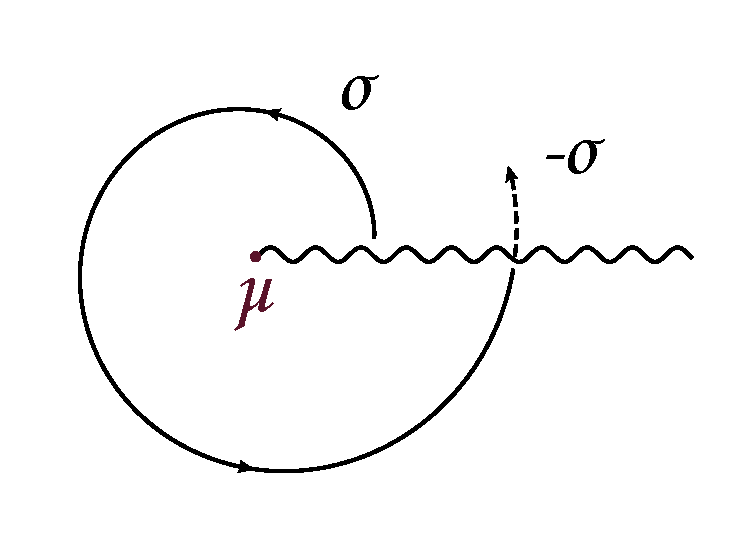
\includegraphics[width=6cm]{picture/order-disorder}
\end{figure}

In fact, identifying the various operators in Ising model with the primaries in  $\cM_{p=3}$
\bea
\psi (z)& \sim\phi _{2,1} (z) \otimes \phi _{1,1} (\overline{z}) \cr \overline{\psi} (\overline{z})& \sim\phi _{1,1} (z) \otimes \phi _{2,1} (\overline{z}) \cr
\psi \overline{\psi} : =\varepsilon (z , \overline{z})&\sim \phi _{2,1} (z) \otimes \phi _{2,1} (\overline{z})\cr
 \sigma (z , \overline{z}) \ \textrm{or} \ \mu (z , \overline{z}) &\sim\phi _{1,2} (z) \otimes \phi _{1,2} (\overline{z})
 \eea
we obtain desired OPE relations. Note that $\sigma$ and $\mu$ have the same conformal dimension because the Kramers-Wannier duality exchanges the spin and disorder operator $\sigma\leftrightarrow\mu$. The fusion rule in $\cM_{p=3}$ can be read off as
\begin{equation}
  \sigma \times \sigma=\mathbf{1} + \varepsilon ~,\qquad  \varepsilon \times \varepsilon=\mathbf{1} ~,\qquad  \sigma \times \varepsilon=\sigma~.
\end{equation}


Moreover, using the associativity of OPEs, one can derive from \eqref{sigma-mu}
\[
\psi ( z ) \sigma ( w,\overline w ) \sim \frac{1}{( z - w ) ^ { \frac12}} \mu ( w ,\overline w)~.
\]
We can compare this with the mode expansion of free fermion on the Ramond sector
\[
\psi ( z ) \sigma ( 0 ) = \sum _ { r \in \bZ} z ^ { - r - \frac12} b _ { r} \sigma ( 0 )~,
\]
we can deduce
\begin{equation}b _ { 0} \sigma ( 0 ) = \mu ( 0 )~.\end{equation}
In the presence of the spin field $\sigma(0)$ at the origin, the fermion field obeys the anti-periodic boundary condition
\[\psi ( z ) \rightarrow \psi ( e ^ { 2 \pi i} z ) = - \psi ( z )~.\]
The spin field $\sigma$ creates a branch cut, which changes the boundary condition of the fermion field. Hence, $\sigma$ can be regarded as the \textbf{twist operator}.

Finally, let us consider the partition functions of the Ising model. There are three unitary irreducible representations corresponding to the highest weights  $h=0,\frac12,\frac1{16}$, and the corresponding characters can be read off from \eqref{Rocha-Caridi-formula} as
\begin{gather}
\chi_{0}=\frac12 \left(\sqrt{\frac{\vartheta_3}{\eta}}+\sqrt{\frac{\vartheta_4}{\eta}} \right)=\mbox{Tr}_{NS}\left(\frac{1+(-1)^F}{2}q^{L_0-\frac{c}{24}} \right), \nonumber \\
\chi_{\frac12}=\frac12 \left(\sqrt{\frac{\vartheta_3}{\eta}}-\sqrt{\frac{\vartheta_4}{\eta}} \right)=\mbox{Tr}_{NS}\left(\frac{1-(-1)^F}{2}q^{L_0-\frac{c}{24}} \right), \\
\chi_{\frac{1}{16}}=\frac{1}{\sqrt{2}} \sqrt{\frac{\vartheta_2}{\eta}}=\mbox{Tr}_{R}\left(q^{L_0-\frac{c}{24}} \right). \nonumber
\end{gather}
Using these expressions, the partition function of the Ising model of diagonal type is equal to that of the free fermion \eqref{free-fermion-PF}
\begin{equation}\label{free-fermion-minimal-model}
\cZ_{\textrm{F}}(\tau, \overline{\tau})=\chi_0\overline{\chi}_0+\chi_{\frac{1}{2}}\overline{\chi}_{\frac{1}{2}}+\chi_{\frac{1}{16}}\overline{\chi}_{\frac{1}{16}}.
\end{equation}
The structure of this partition function also appears when studying superstrings, and the operator $\frac12 (1+(-1)^F)$ is known as the \textbf{Gliozzi-Scherk-Olive (GSO) projection}.

\subsection{Other examples}\label{sec:examples}

\subsubsection*{Yang-Lee singularity $(p',p)=(2,5)$}
Among the minimal non-unitary models, a simple but particularly significant example is given by the model $\cM_{2,5}$ with central charge is $c=-22/5$.  The primary fields in the theory are identity operator and a field $\phi_{1,2}$ of conformal dimension $h=-1/5$.



The partition function of a statistical model defined on a lattice is an analytic function of its parameters as long as the number $N$ of the fluctuating variables is finite. Let us consider the Ising model at a given temperature $T$  in the presence of an external magnetic field $B$
\begin{equation}\mathcal{H}=- J \sum _{\left\langle i ,\right\rangle} \sigma _{i} \sigma _{j}-B \sum _{i} \sigma _{i}\end{equation}
The Yang-Lee theorem states that the zeroes of the partition function $Z$ are all on the imaginary axis $\Re B=0$. Fisher showed that the points $B=\pm iB_c$ are new critical points of the theory, which are called \textbf{Yang-Lee edge singularities}. Furthermore, he has argued that the effective action is given by the Landau-Ginzburg theory
\[
\mathcal{S}=\int d^{2} z \left[ \frac{1}{2} (\partial \Sigma)^{2} + i \left(B-B _{c} \right) \Sigma + i g \Sigma^{3} \right]
\]
where the non-unitarity of the model manifests itself in the imaginary value of the coupling constant.  This model is described by the non-unitary minimal  model $\cM_{2,5}$ \cite[ISZ88-No.13]{Cardy:1985yy}.

\subsubsection*{Tricritical Ising model $(p',p)=(5,4)$}


\begin{table}[htbp]\centering
\begin{tabular}{c|ccc}
		$4$
		& $\frac32$
		& $\frac72$
		& $0$
		\\ [5pt]
		$3$
		& $\frac35$
		& $\frac3{80}$
		& $\frac1{10}$
		\\[5pt]
		$2$
		& $\frac1{10}$
		& $\frac3{80}$
		& $\frac35$
		\\[5pt]
		$1$
		& $0$
		& $\frac7{16}$
		& $\frac32$
		\\    [5pt]
		\midrule
		$0$
		& $1$
		& $2$
		& $3$
	\end{tabular}\hspace{2cm}
\begin{tabular}{c|ccc}
				$4$
		& $G$
		& $\sigma'$
		& $\mathbf{1}$
		\\ [5pt]
		$3$
		& $t$
		& $\sigma$
		& $\varepsilon$
		\\[5pt]
		$2$
		& $\varepsilon$
		& $\sigma$
		& $t$
		\\[5pt]
		$1$
		& $\mathbf{1}$
		& $\sigma'$
		& $G$
		\\    [5pt]
		\midrule
		$0$
		& $1$
		& $2$
		& $3$
		\end{tabular}\label{Tab-Min4}
\end{table}


Let us consider the variant of the Ising model whose Hamiltonian is given by
\[
\mathcal{H}=- J \sum _{\langle i , j \rangle}^{N} \sigma_{i} \sigma_{j} t _{i} t _{j}- B \sum _{i=1}^{N} \sigma_{i} t _{i}-\mu \sum _{i=1}^{N} t _{i}
\]
where a spin variable $\sigma_k$ takes values $\pm1$, and a vacancy variable $t_k$, with values $0$ and $1$. This variable specifies whether the site
is empty (0) or occupied (1). The chemical potential $\mu$ controls the density of the vacancy.


\begin{figure}[ht]\centering
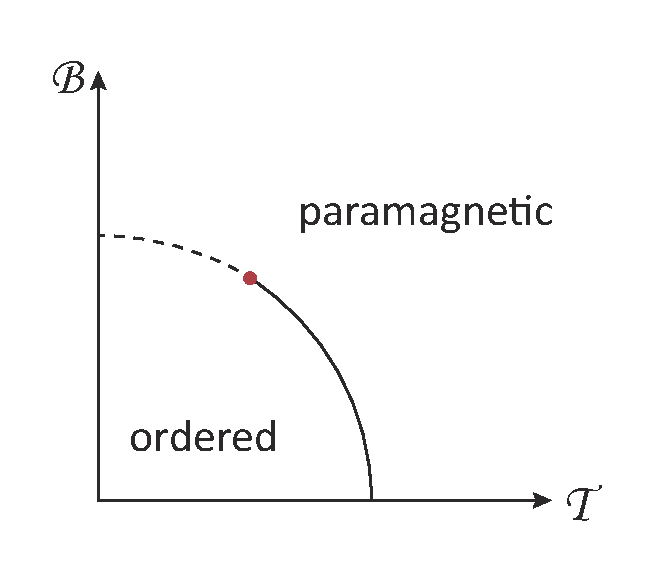
\includegraphics[width=7cm]{picture/tricritical}
\caption{Phase diagram of the tricritical Ising model. The (broken) first-order line and the (full) line of Ising critical points meet at the tricritical point $(B_t, T_t)$, shown as a black dot}\label{fig:tricritical}
\end{figure}


A typical phase diagram of this model is sketched in Figure \ref{fig:tricritical}, where the lines of first-order and second-order transitions meet in the tricritical point, located at $B=B_t$ and $T=T_t$. While at a normal critical point the two phases become indistinguishable, at a tricritical point three physically distinct phases merge. For that reason, this model is called the \textbf{tricritical Ising model}. The phenomenology of the tricritical Ising model is described in \cite[\S4]{cardy1996scaling}.


Remarkably, the tricritical model is described by $\cN=1$ superconformal field theory where $G$ is the supercurrent \cite[ISZ88-No.5]{friedan1985superconformal}.



\subsubsection*{3-state Potts model $(p',p)=(6,5)$}
\[\begin{array}{c| c c  c  c } 5& 3 &{\frac{7}{5}} &{\frac{2}{5}} &{0} \\[5pt] 4& \frac{13}{8} &{\frac{21}{40}} &{\frac{1}{40}} &{\frac{1}{8}} \\[5pt] 3&  \frac{2}{3} &{\frac{1}{15}} &{\frac{1}{15}} &{\frac{2}{3}} \\[5pt] 2& \frac{1}{8} &{\frac{1}{40}} &{\frac{21}{40}} &{\frac{13}{8}} \\[5pt] 1& 0 &{\frac{2}{5}} &{\frac{7}{5}} &{3} \\[5pt] \hline &1&2&3&4  \end{array}\]

On a square lattice, the hamiltonian of the three-state Potts model is given by
\begin{equation}\cH=- \frac{J}{2} \sum _{\langle i, j \rangle} \left(\sigma _{i} \overline{\sigma} _{j} + \overline{\sigma} _{i} \sigma _{j} \right)
\end{equation}
where $\sigma$ takes the values $\omega^i$ (i=1,2,3) with a third root of unity $\omega=e^{2\pi i/3}$. This model undergoes a second-order phase transition at $J_c=\frac{2}{3} \log (\sqrt{3} + 1)$, which is endowed with the $\bZ_3$ symmetry  \cite[ISZ88-No.12]{dotsenko1984critical}. The lattice theory is exactly solvable and consequently all critical exponents are known. For instance,
\[
h_{\sigma}=h_{\overline \sigma}=\frac1{15}~,\qquad h_\varepsilon=\frac{2}{5}~.
\]
It is tempting to identify the primary field of the unitary minimal model $\cM_{p=5}$.
However, the exact solution of the lattice model does not have operators with
conformal dimensions $\frac18$, $\frac1{40}$, $\frac{21}{40}$, and $\frac{13}8$  \cite[ISZ88-No.22]{vonGehlen:1986gk}.


In fact, the partition function of  the 3-state Potts model  is described by the non-diagonal type
\be\label{3-state-Potts}
\cZ _{\text{3-Potts}}=\sum _{r=1,2} \left\{\left| \chi _{r , 1} + \chi _{r , 5} \right|^{2} + 2 \left| \chi _{r , 3} \right|^{2} \right\}~,
\ee
so that the primary fields are
\[
(0,0) , \left(\frac{2}{5} , \frac{2}{5} \right) , \left(\frac{7}{5} , \frac{7}{5} \right)~, 2 \times \left(\frac{1}{15} , \frac{1}{15} \right) , 2 \times \left(\frac{2}{3} , \frac{2}{3} \right)  (0,3) , (3,0) , \left(\frac{2}{5} , \frac{7}{5} \right) , \left(\frac{7}{5} , \frac{2}{5} \right)
\]
It is noteworthy that there are chiral spin-3 currents $W(z)$ and $\overline W(\overline z)$ corresponding to  (0,3), (3,0)  \cite[ISZ88-No.6]{Zamolodchikov:1985wn}. In fact, $W(z)$ with the energy momentum tensor $T(z)$ forms $W_3$-algebra \cite{Fateev:1987vh}.


\subsubsection*{Other models}

It was shown in \cite[ISZ88-No.32]{Huse:1984mn} that a general unitary minimal model $\cM_p$ of diagonal type describes an RSOS model constructed in \cite[ISZ88-No.31]{Andrews:1984af}.
Furthermore, the CFT with $\bZ_k$ symmetry has been constructed in \cite[ISZ88-No.14]{fateev1985parafermionic}, which we will see in \S\ref{sec:coset}, where the central charge is
\be\label{Zk-cc} c = \frac { 2 ( k - 1 )} { k + 2}~.\ee
When $k=4$, the central charge is $c=1$ and the corresponding CFT is called the \textbf{Ashkin-Teller model} where the Hamiltonian is written by the two spin fields $ \sigma _ { i} $ and $ \tau _ { i} $ as
\[\mathcal { H} = - J _ { 2} \sum _ { \langle i , j \rangle} \left( \sigma _ { i} \sigma _ { j} + \tau _ { i} \tau _ { j} \right) - J _ { 4} \sum _ { \langle i , j \rangle} \sigma _ { i} \sigma _ { j} \tau _ { i} \tau _ { j}~.\]
The $\bZ_4$ symmetry is given by
\[
s_j\to e^{\frac{i\pi k}{2}}s_j ~, \qquad \textrm{where}\qquad
s_j\equiv \frac{\sigma _ { j} +i\tau _ { j}}{\sqrt{2}}~.
\]
This Ashkin-Teller model can be described by the free boson on an orbifold space $S^1/\bZ_2$, which will be studied in \S\ref{sec:orbif-part-funct}.
All in all, these models are the main characters in the papers listed in \cite{itzykson1988conformal}.









\subsection{Conformal blocks and bootstrap}\label{sec:bootstrap}
\subsubsection*{The Operator Algebra}
The main object of a field theory is the calculation of correlation functions. We have seen the forms of two- and three-point functions in \eqref{two-point-func-form} and \eqref{three-point-func-form}. As mentioned before, one way to construct all correlation functions is to find the corresponding operator algebra: The complete OPE (including all regular terms) of all primary fields with each other.
So far, we consider the fusion rule of primary fields in a minimal model, which does not tell anything about the coefficients of operator algebra. This section aims to spell out the coefficients of operator algebra and conformal bootstrap approach.

Let us start with a two-point function.
Since the coefficient $C_{12}$ of a two-point function \eqref{two-point-func-form} is symmetric,  we are free to choose a basis of primary fields of conformal dimension $h$ so that $C_{\alpha\beta}=\delta_{\alpha\beta}$. Thus, conformal families associated with different $\phi_\alpha$ are orthogonal in the sense of the two-point function.

The general form of OPE of primary fields is given in
\eqref{op-algebra}. In fact, the three-point function \eqref{three-point-func-form} explicitly determines the coefficient of the most singular term of the OPE \eqref{op-algebra} as $C _{12p}^{\{0,0 \}}= C _{12p}$. Moreover,
since the correlations of descendants are built on the correlation of the primaries as in \eqref{descendant-eq}, we expect the coefficient to have the form:
\begin{equation}
C^{\{k,\overline{k}\}}_{12p}=C_{12p}
\beta^{p\{k\}}_{12}
\overline{\beta}^{p\{\overline{k}\}}_{12}\, .
\end{equation}
where $\beta^{p\{k\}}_{ij}$ can be determined by the descendant equation \eqref{descendant-eq} as functions of central charge $c$ and of conformal dimensions.
Therefore, once we find all the coefficients $C_{pnm}$ of three-point functions with primary fields, we determine all OPEs. Indeed, the conformal bootstrap is one powerful way to determine  $C_{pnm}$.

\subsubsection*{Conformal Blocks}
To explain the conformal bootstrap, let us consider a four-point:
\begin{equation}
\left\langle \phi _{1} \left(z _{1} , \overline{z} _{1} \right) \phi _{2} \left(z _{2} , \overline{z} _{2} \right) \phi _{3} \left(z _{3} , \overline{z} _{3} \right) \phi _{4} \left(z _{4} , \overline{z} _{4} \right) \right\rangle\,,
\end{equation}
By a suitable conformal transformation, we can set $z_4 =0, z_1=\infty, z_2=1$ and $z_3 =x$ where $x$ is the cross-ratio of $z_{1,2,3,4}$:
\begin{equation}
G _{34}^{21} (x , \overline{x}) =
\lim _{z _{1} , \overline{z} _{1} \rightarrow \infty} z _{1}^{2 h _{1}} \overline{z} _{1}^{2\overline{h} _{1}} \left\langle \phi _{1} \left(z _{1} , \overline{z} _{1} \right) \phi _{2} (1,1) \phi _{3} (x , \overline{x}) \phi _{4} (0,0) \right\rangle\, ,
\end{equation}
Applying the operator algebra \eqref{op-algebra} to
$\phi_3(x,\overline{x})\phi_4(0,0)$ ,
the function $G^{21}_{34}$ becomes
\begin{equation}\label{four-point}
G _{34}^{21} (x , \overline{x})=\sum _{p} C_{12p}C_{34p}  \mathcal{F} _{34}^{21} (p | x) \overline{\mathcal{F}} _{34}^{21} (p | \overline{x})\, ,
\end{equation}
where
\begin{equation}
\label{conformal-block}
\mathcal{F} _{34}^{21} (p | x)=x^{h _{p}-h _{3}-h _{4}} \sum _{\{k \}} \beta _{34}^{p (k)} x^{K} \frac{\left\langle h _{1} \left| \phi _{2} (1) L _{- k _{1}} \cdots L _{- k _{N}} \right| h _{p} \right\rangle}{\left\langle h _{1} \left| \phi _{2} (1) \right| h _{p} \right\rangle}\, ,
\end{equation}
which are called \textbf{conformal blocks}. The denominator is simply equal to $(C_{12p})^{\frac12}$. They can be simply calculated by commuting the Virasoro generators over the field $\phi_2(1)$, and can be represented in terms of central charge and conformal dimensions. Since we fuse $\phi_3$ and $\phi_4$ to produce intermediate operators $[\phi_p]$, and $[\phi_p]$ then interact with $\phi_1$ and $\phi_2$, this process can be displayed as in Figure  \ref{fig:tree}.
\begin{figure}[ht]
	\centering
	\includegraphics[width=0.6\linewidth]{picture/tree}
	\caption{Diagram for the conformal block}
	\label{fig:tree}
\end{figure}

By expanding the conformal block as a power of the cross-ratio $x$
series in $x$:
\begin{equation}
\mathcal{F} _{34}^{21} (p | x)=x^{h _{p}-h _{3}-h _{4}} \sum _{K=0}^{\infty} \mathcal{F} _{K} x^{K}\,.
\end{equation}
we can present several leading coefficients
\eqref{conformal-block}.
\begin{equation}
\mathcal{F}_{0}=1\, , \qquad
\mathcal{F} _{1}=\frac{\left(h _{p} + h _{2}-h _{1} \right) \left(h _{p} + h _{3}-h _{4} \right)}{2 h _{p}}
\end{equation}
\bea
\mathcal{F} _{2} &= \frac{\left(h _{p} + h _{2}-h _{1} \right) \left(h _{p} + h _{2}-h _{1} + 1 \right) \left(h + h _{3}-h _{4} \right) \left(h + h _{3}-h _{4} + 1 \right)}{4 h _{p} \left(2 h _{p} + 1 \right)}\notag\\
&+ 2 \left(\frac{h _{1} + h _{2}}{2} + \frac{h _{p} \left(h _{p}-1 \right)}{2 \left(2 h _{p} + 1 \right)}-\frac{3 \left(h _{1}-h _{2} \right)^{2}}{2 \left(2 h _{p} + 1 \right)} \right)^{2}\notag\\
&
\times \left(\frac{h _{3} + h _{4}}{2} + \frac{h _{p} \left(h _{p}-1 \right)}{2 \left(2 h _{p} + 1 \right)}-\frac{3 \left(h _{3}-h _{4} \right)^{2}}{2 \left(2 h _{p} + 1 \right)} \right)^{2} \left(c + \frac{2 h _{p} \left(8 h _{p}-5 \right)}{2 h _{p} + 1} \right)^{- 1}
\eea

\subsubsection*{Crossing Symmetry and the Conformal Bootstrap}
To obtain a four-point function, we fuse $\phi_3$ and $\phi_4$ in \eqref{four-point}. However, we can also take different pairs for a fusion, say  $\phi_3$ and $\phi_2$. For this, we can send $z_2$ to $0$ and $z_4$ to $1$, and then $z_3$ proves to be $1-x$. Then, the same procedure will give a different basis $\mathcal{F} _{32}^{41} (q | 1-x)$ of conformal blocks. Nonetheless, the final result for the four-point function should be the same
\begin{equation}
\label{Bootstrap method}
G^{21}_{34}(x,\overline{x})=G^{41}_{32}(1-x,1-\overline{x})
\, ,
\end{equation}
which implies
\begin{equation}\label{bootstrap}
\sum _{p} C _{12p} C _{34p} \mathcal{F} _{34}^{21} (p | x) \overline{\mathcal{F}} _{34}^{21} (p | \overline{x})=
\sum _{q} C _{14q} C _{23q} \mathcal{F} _{32}^{41} (q | 1-x) \overline{\mathcal{F}} _{32}^{41} (q | 1-\overline{x})
\end{equation}
This relation is represented graphically in Figure \ref{fig:crossing-symmetry}

\begin{figure}[ht]
	\centering
	\includegraphics[width=0.8\linewidth]{picture/crossing-symmetry}
	\caption{Crossing symmetry}
	\label{fig:crossing-symmetry}
\end{figure}

If the conformal block $\mathcal{F}$ is known, then \eqref{Bootstrap method} yields a system of equations that can determine $C_{ijk}$'s and $h,\overline{h}$'s. The program of calculating the correlation functions simply by assuming crossing symmetry is known as the \textbf{conformal bootstrap} approach. For minimal models, the bootstrap equations can be solved completely.


\end{document}
